\documentclass[9pt,twocolumn,twoside]{pnas-new}
% Use the lineno option to display guide line numbers if required.
% Note that the use of elements such as single-column equations
% may affect the guide line number alignment. 

\templatetype{pnasresearcharticle} % Choose template 
% {pnasresearcharticle} = Template for a two-column research article
% {pnasmathematics} = Template for a one-column mathematics article
% {pnasinvited} = Template for a PNAS invited submission

\title{Notes: Ecological Genomics}

% Use letters for affiliations, numbers to show equal authorship (if applicable) and to indicate the corresponding author
\author[a,1]{Matthew K. Lau}

\affil[a]{Harvard Forest, Harvard University, Petersham, MA 01366}

% Please give the surname of the lead author for the running footer
\leadauthor{Lau} 

% Please add here a significance statement to explain the relevance of your work
\significancestatement{

%% Authors must submit a 120-word maximum statement about the
%% significance of their research paper written at a level understandable
%% to an undergraduate educated scientist outside their field of
%% specialty. The primary goal of the Significance Statement is to
%% explain the relevance of the work in broad context to a broad
%% readership. The Significance Statement appears in the paper itself and
%% is required for all research papers.



}

% Please include corresponding author, author contribution and author
% declaration information
\authorcontributions{Please provide details of author contributions here.}
\authordeclaration{Please declare any conflict of interest here.}
\equalauthors{\textsuperscript{1}A.O.(Author One) and A.T. (Author Two) contributed equally to this work (remove if not applicable).}
\correspondingauthor{\textsuperscript{2}To whom correspondence should be addressed. E-mail: author.two\@email.com}

% Keywords are not mandatory, but authors are strongly encouraged to
% provide them. If provided, please include two to five keywords,
% separated by the pipe symbol, e.g:
\keywords{Keyword 1 $|$ Keyword 2 $|$ Keyword 3 $|$ ...} 

\begin{abstract}


%% Please provide an abstract of no more than 250 words in a single
%% paragraph. Abstracts should explain to the general reader the major
%% contributions of the article. References in the abstract must be cited
%% in full within the abstract itself and cited in the text.


\end{abstract}

\dates{This manuscript was compiled on \today}
\doi{\url{www.pnas.org/cgi/doi/10.1073/pnas.XXXXXXXXXX}}

\begin{document}

\section{Ecological Genomics}

\textit{From Van Straalen and Roelofs: Ecological Genomics}

Studies the structure and function of a genome with the aim of understanding the relationship between the organism and its environment.

Genetic turbulance and the entangled bank of the genome.

\textit{2.2} Sequencing genomes

Libraries are collections of all the sequences from a genome fragmented and inserted into a suitable vector, which ideally encompasses the entire genome of the target organism. 

Russel 2002 gives a formula for the number of clones for complete coverage:

n = ln(1 - p) / ln(1-s/G) 

where p = the probability of at least one copy of a DNA fragment is in the library, s is the average insert size and G is the size of the genome. 


\textit{2.2.4} Gene finding and annotation

\begin{itemize}
\item Identify ORFs
\item Codon bias
\item Homolgy search (finding genes)
\item Promoter element association
\item Match with transcript/protein
\item Gene ontology (GO)
\end{itemize}

\textit{2.4} Data analysis

\begin{itemize}
\item Alignment and homology search = BLAST
\end{itemize}

\subsection{Comparing Genomes}

\begin{itemize}
\item Properties of genomes = Genome Size, Gene families, Genomic occurrence (skew, GC content, codon usage), Gene order, Substition patterns
\item See section on Drosophila and other arthropods
\item 
\end{itemize}

\subsection{Microbial Genomics of biogeochemical cycles}

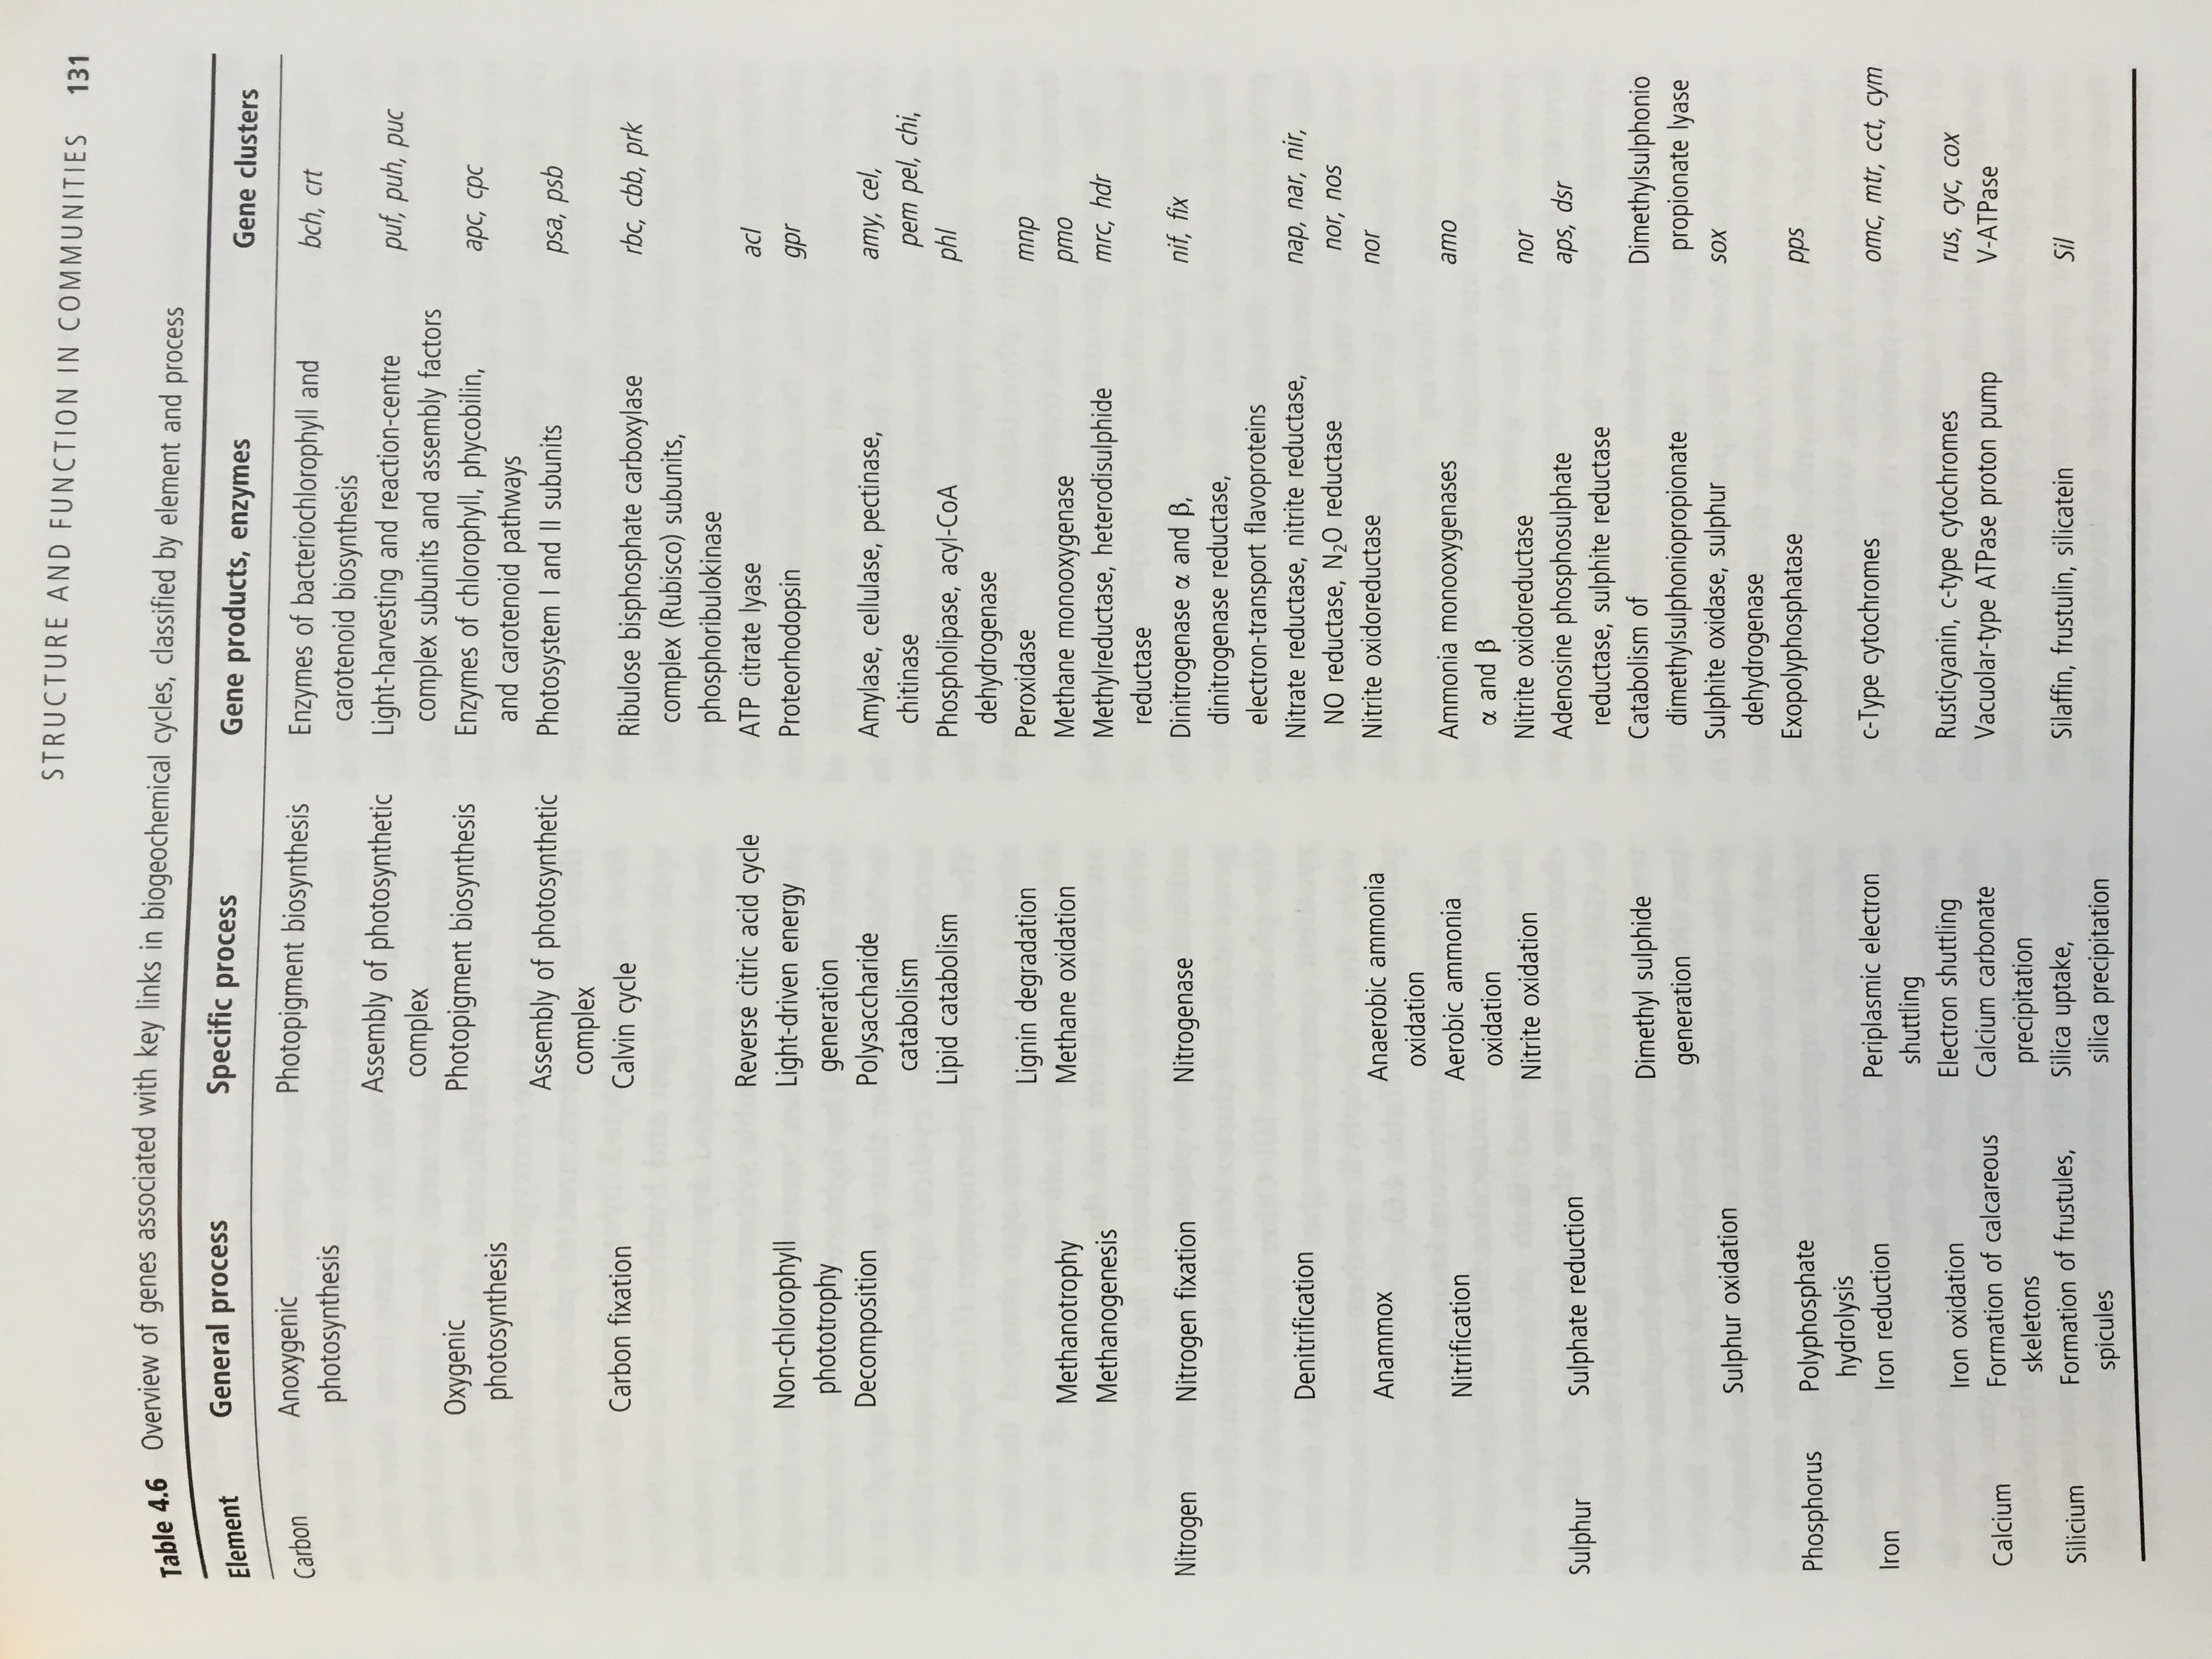
\includegraphics[scale=0.08, angle=-90]{img/ecogenom_tab4_6.jpg}

\subsection{Phenotypic plasticity of life-history traits}

Plastic life-history traits are determined by networks of gene expressions, which integrate multiple cues from the environment with signals from the internal metabolism in such a way that the differences between genes for plasticity and genes for average response cannot be seen.

\textit{Body Size}: Trade-off genes

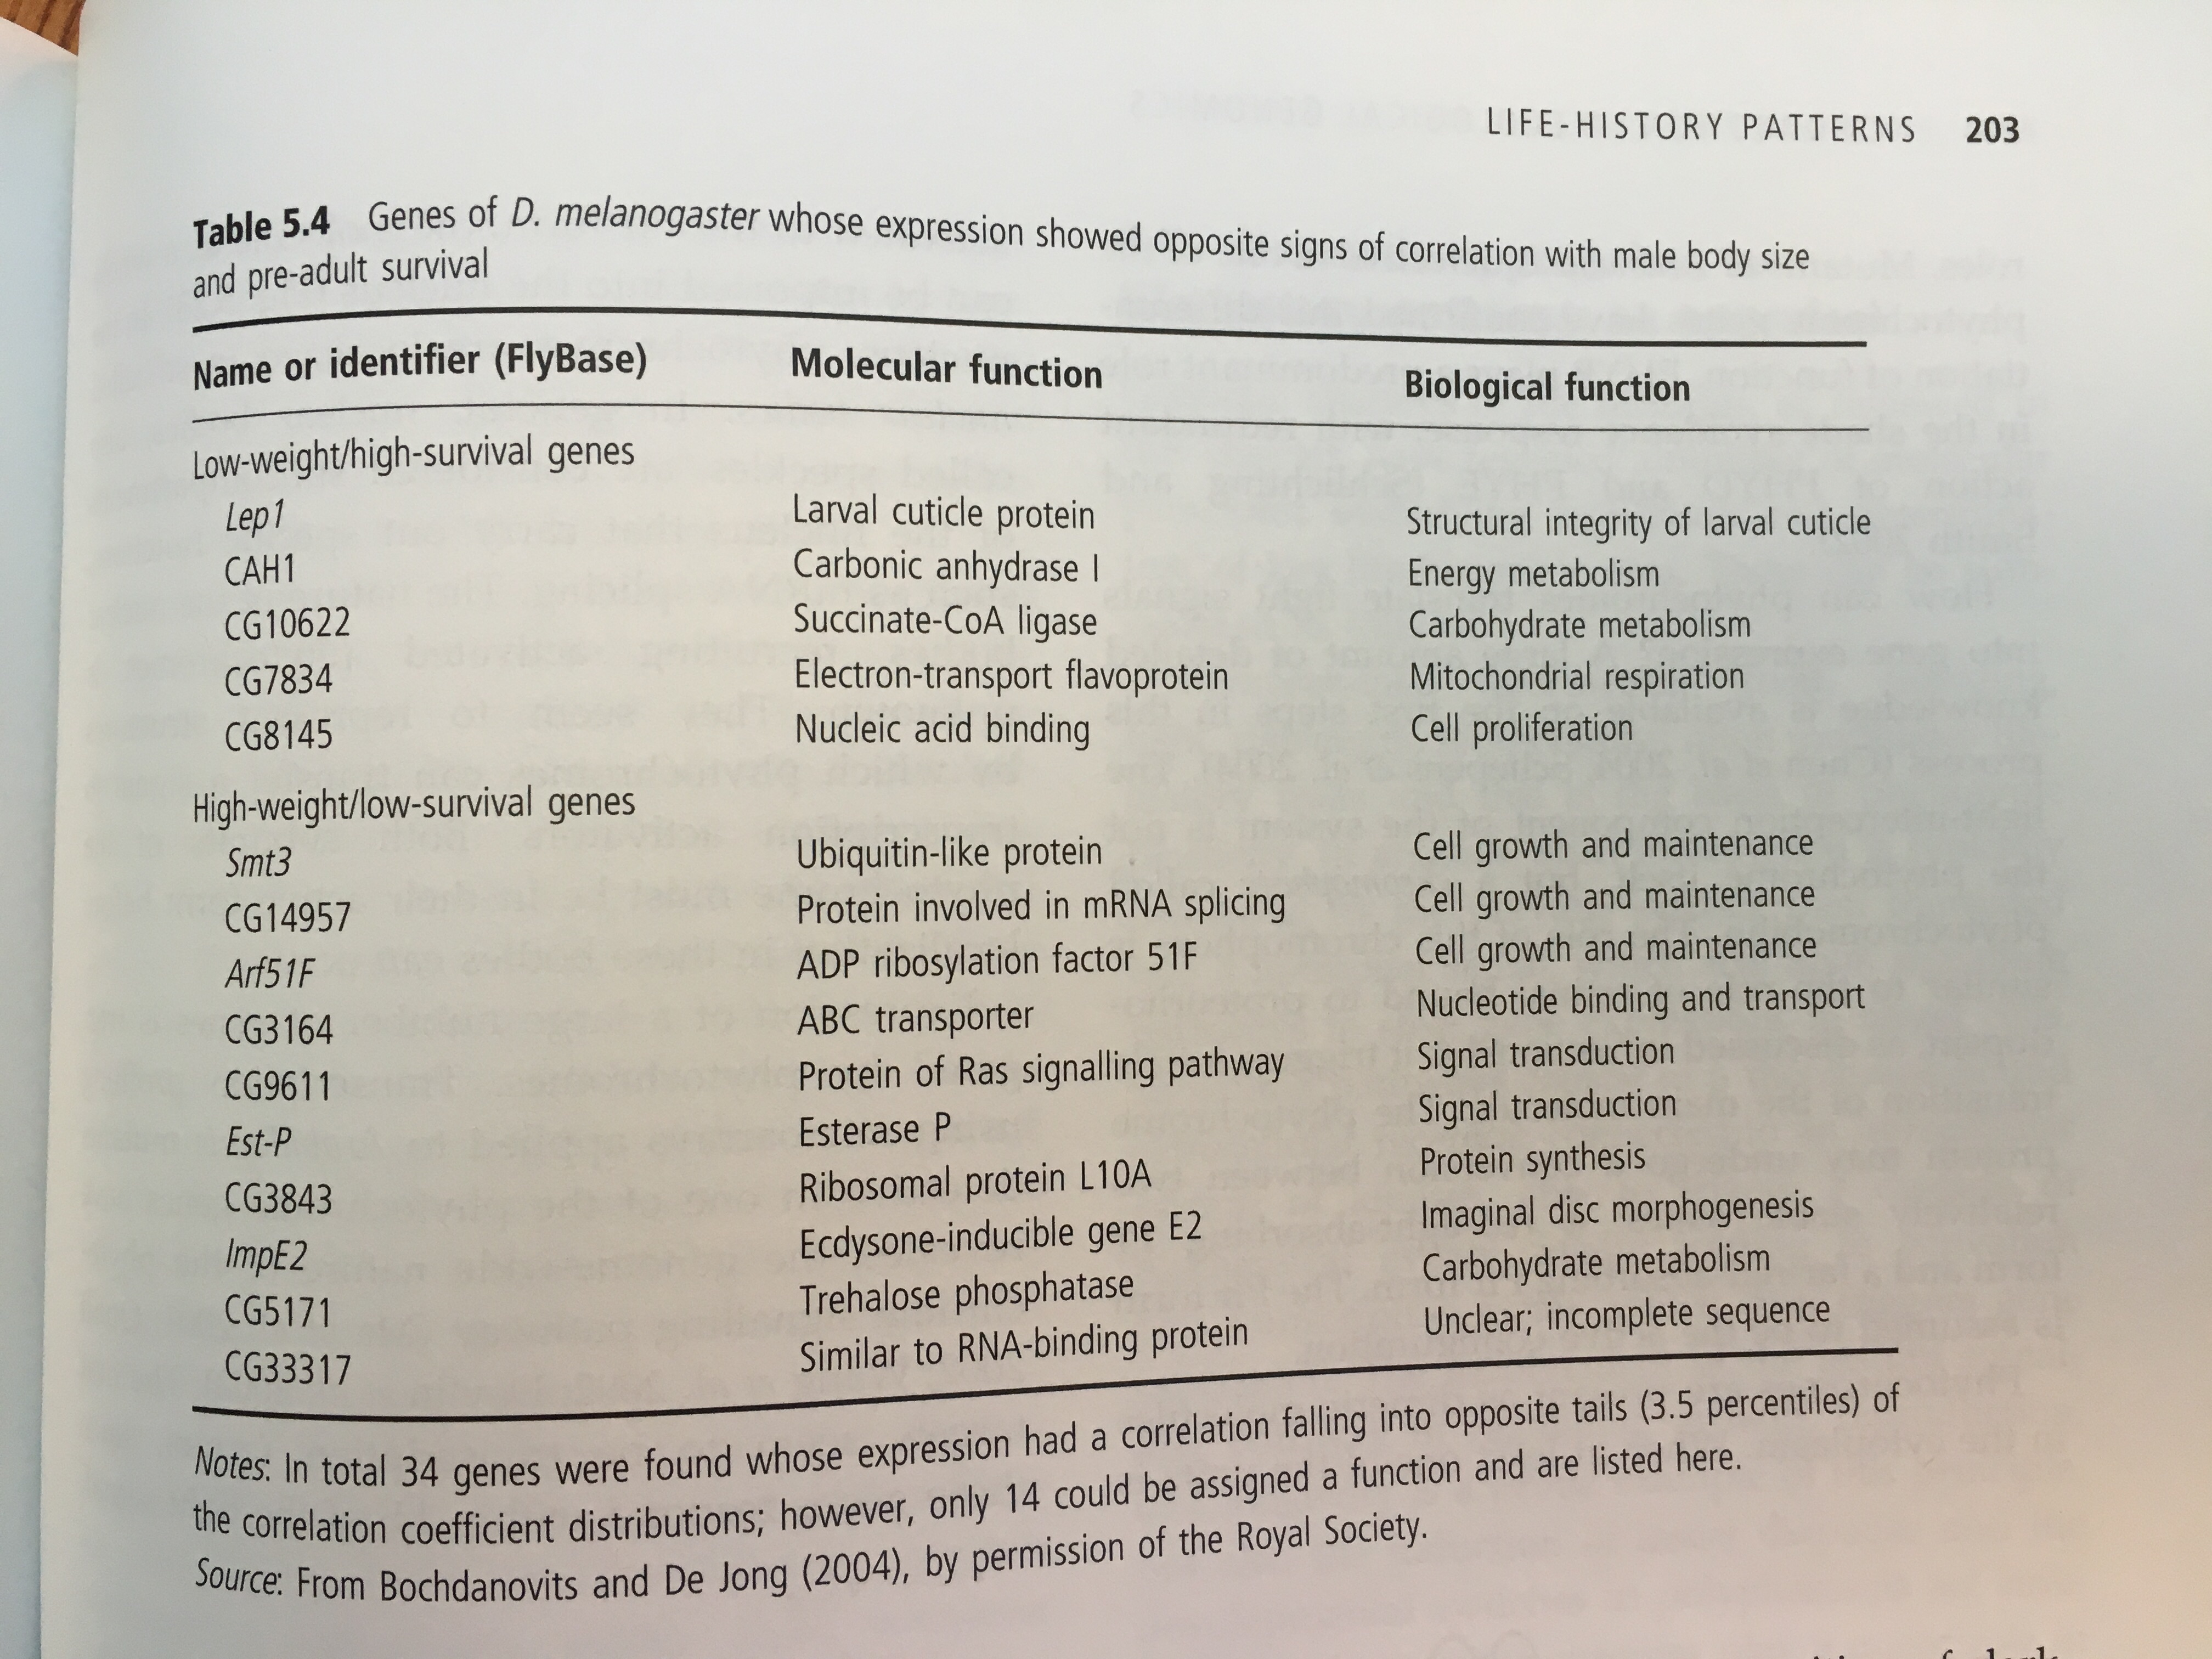
\includegraphics[scale=0.06]{img/ecogenom_tab5_4.jpg}

\textit{Stress Response}: heat-shock proteins, oxidative stress response, 

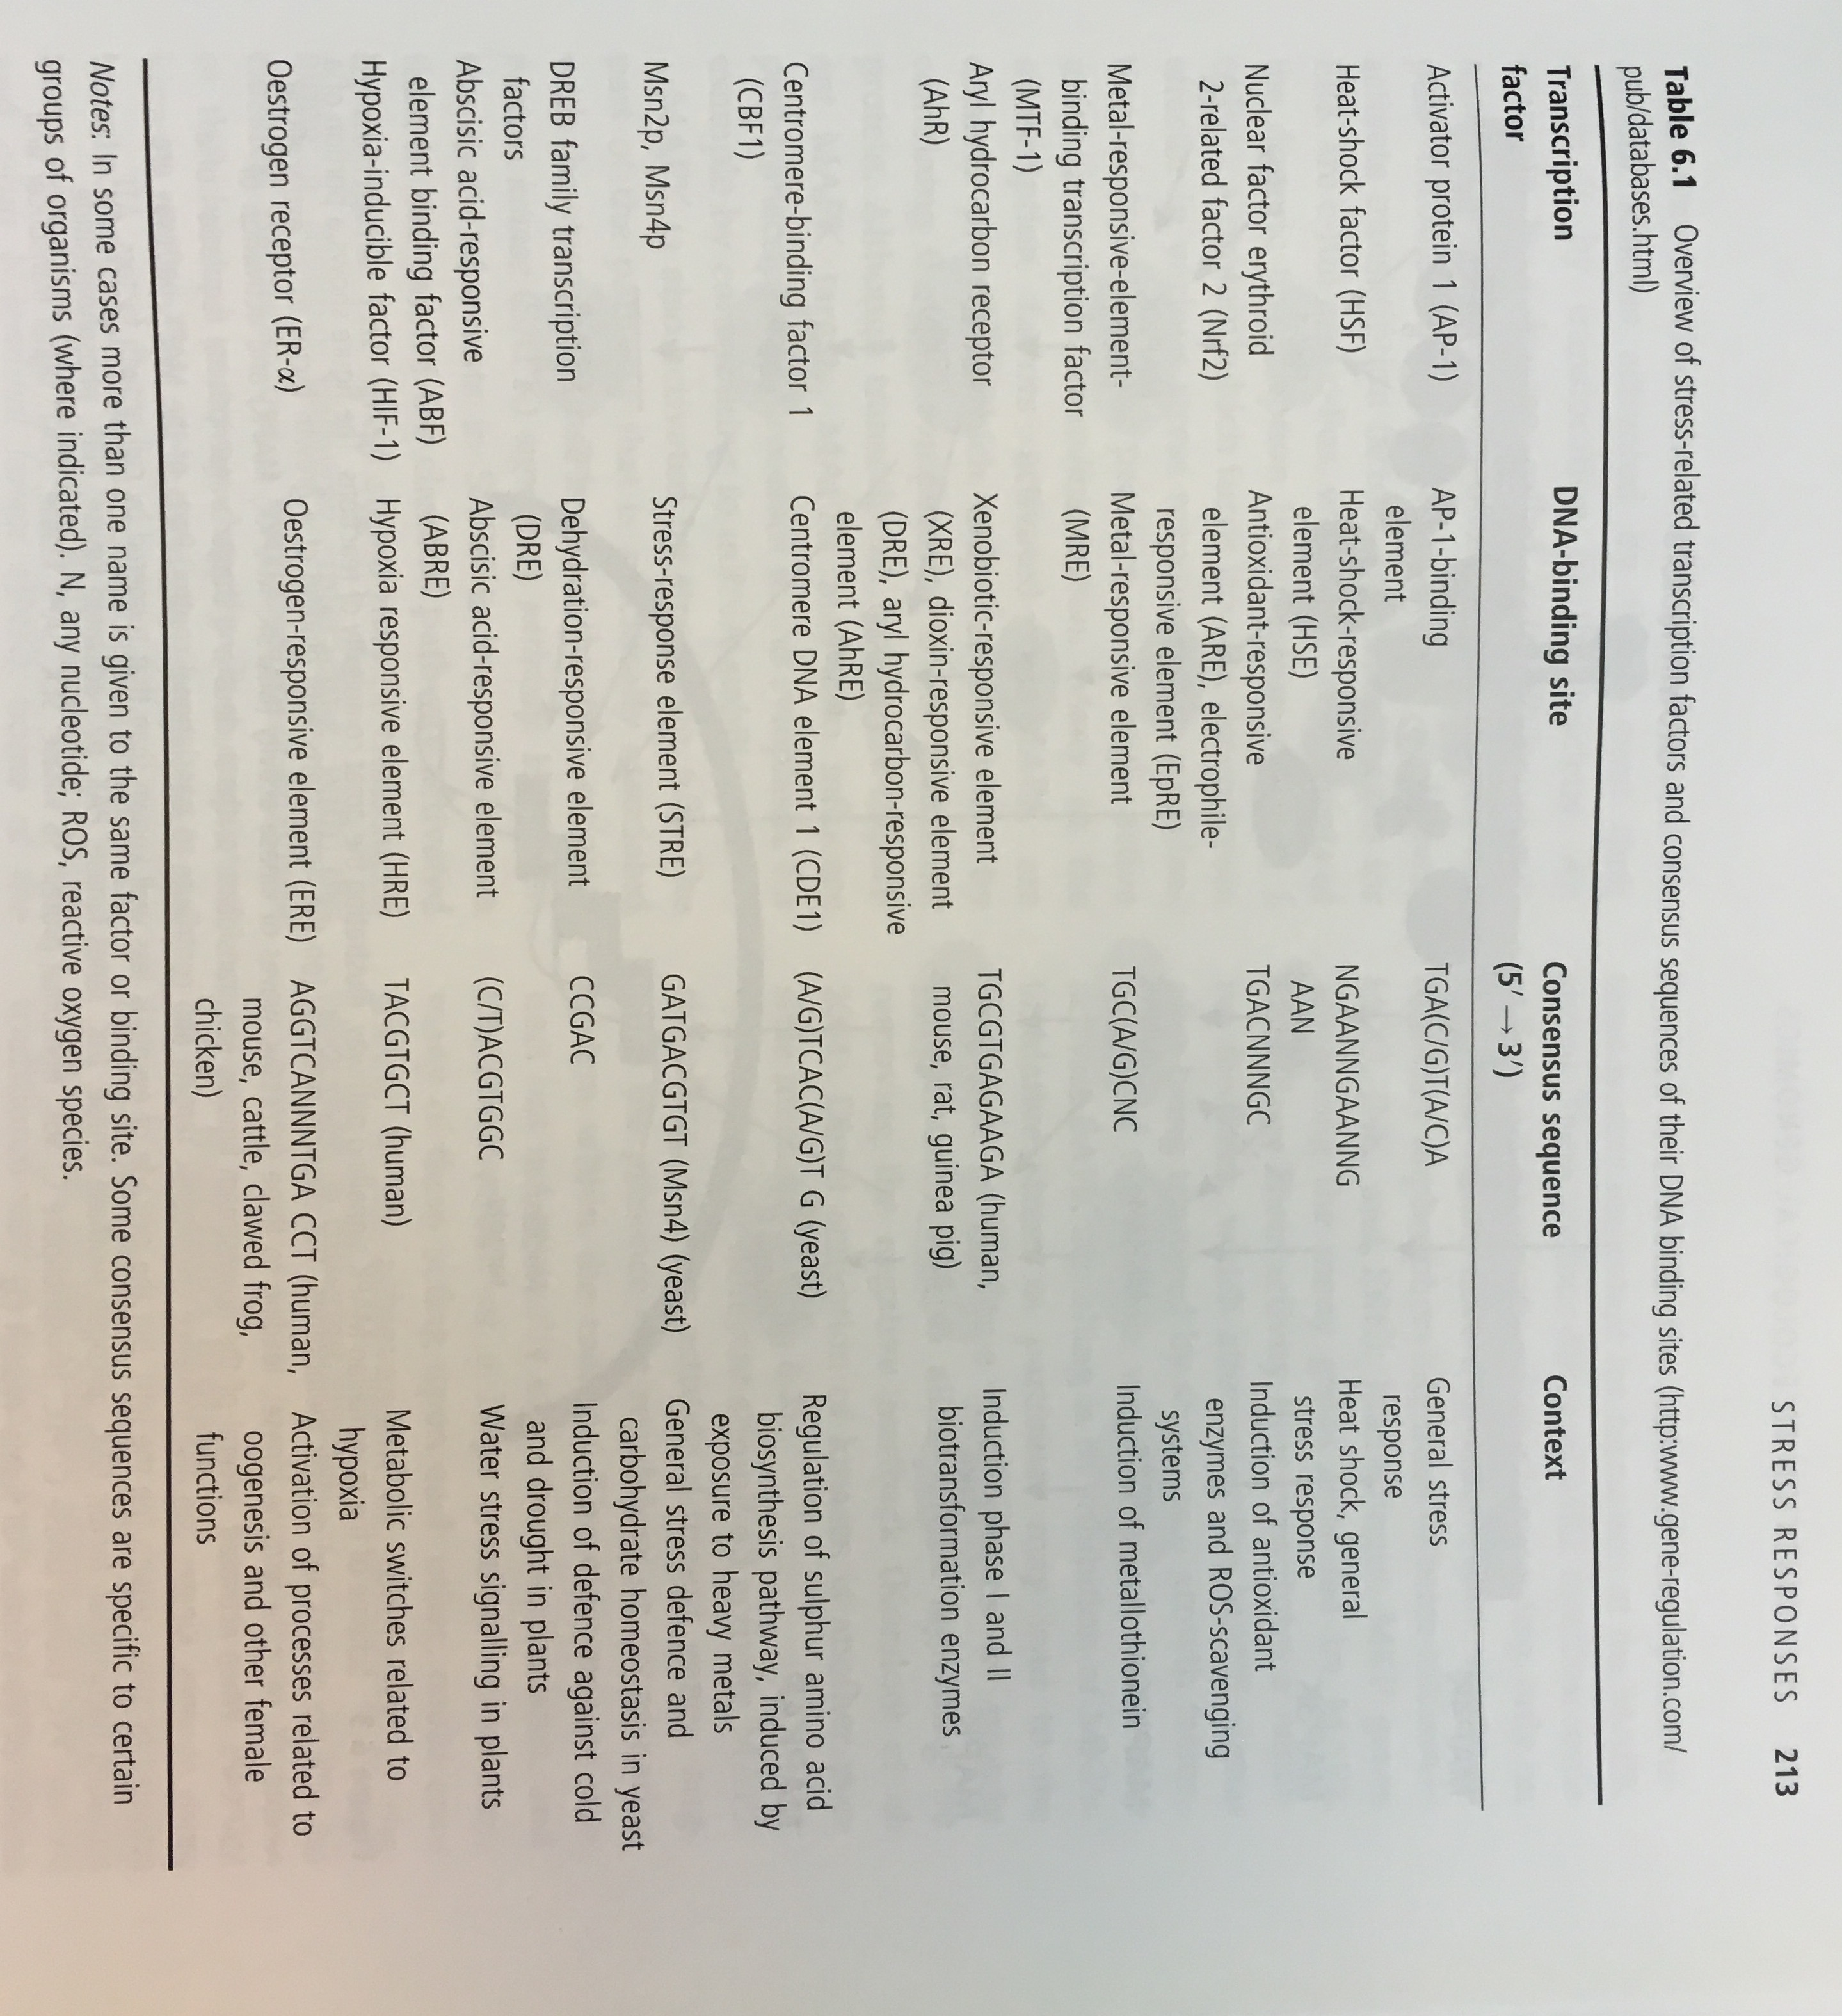
\includegraphics[scale=0.075,angle=90]{img/ecogenom_tab6_1.jpg}

\section{Integrative Ecological Genomics}

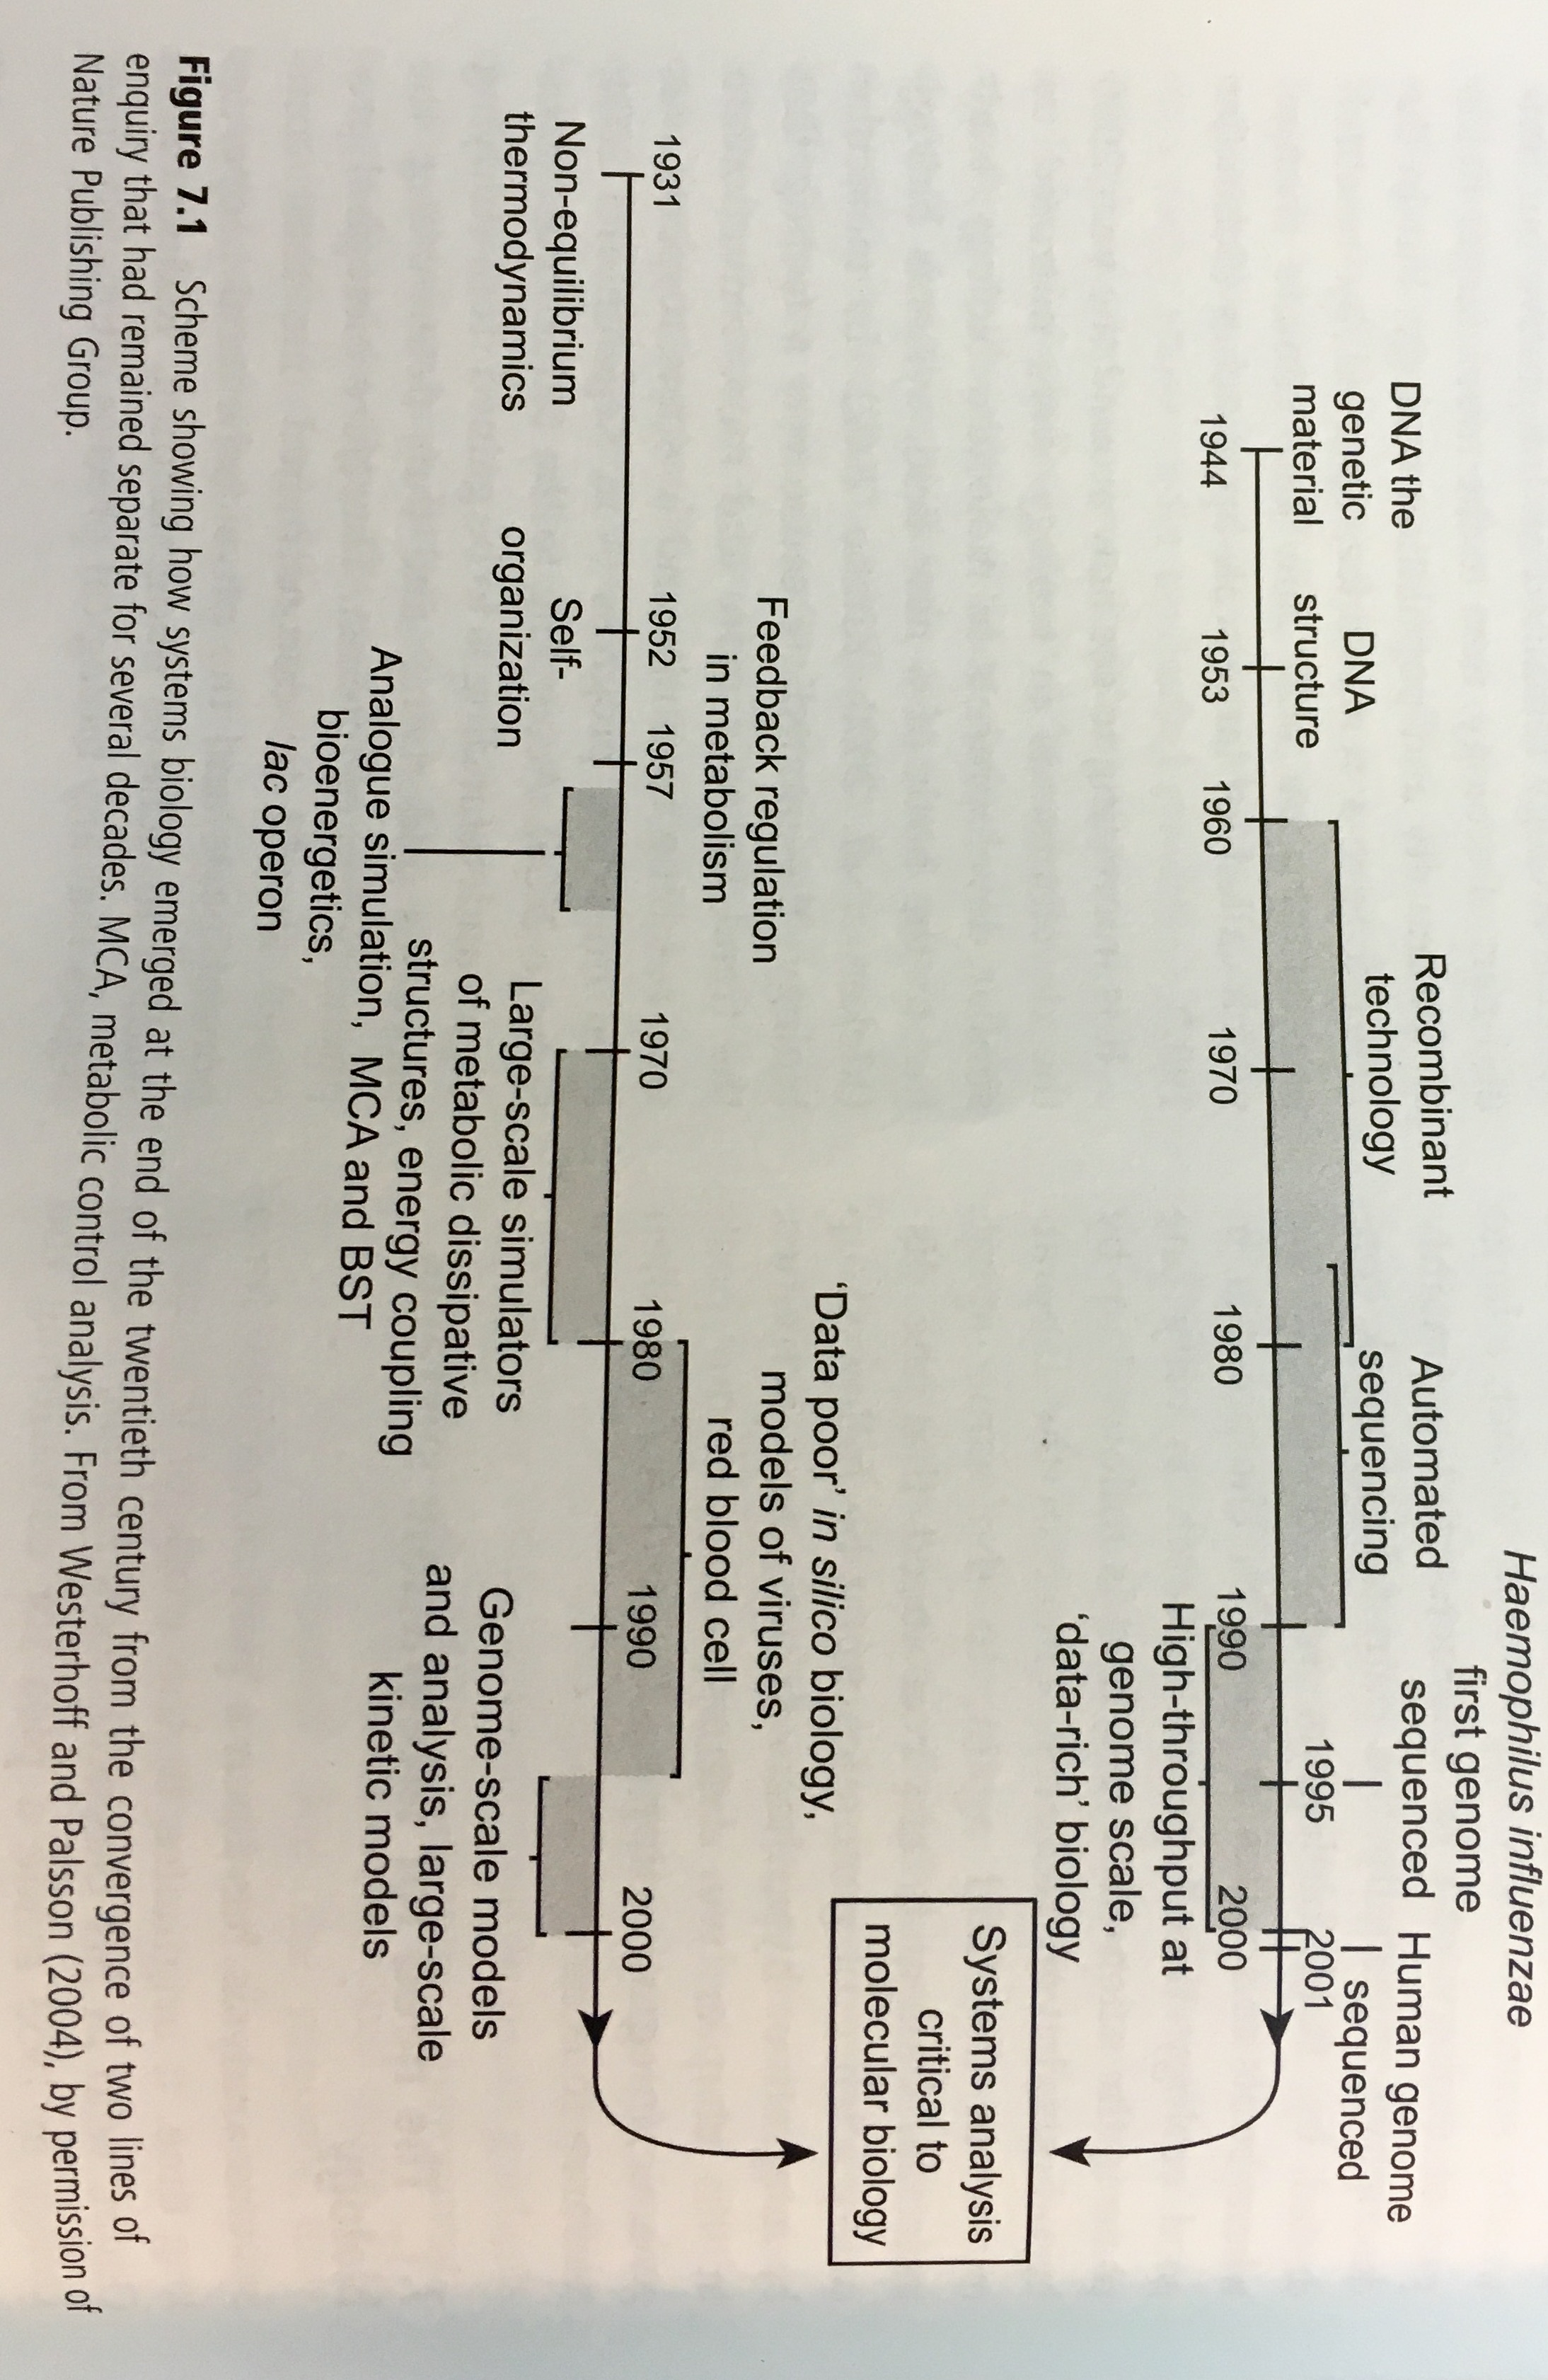
\includegraphics[scale=0.075,angle=90]{img/ecogenom_fig7_1.jpeg}

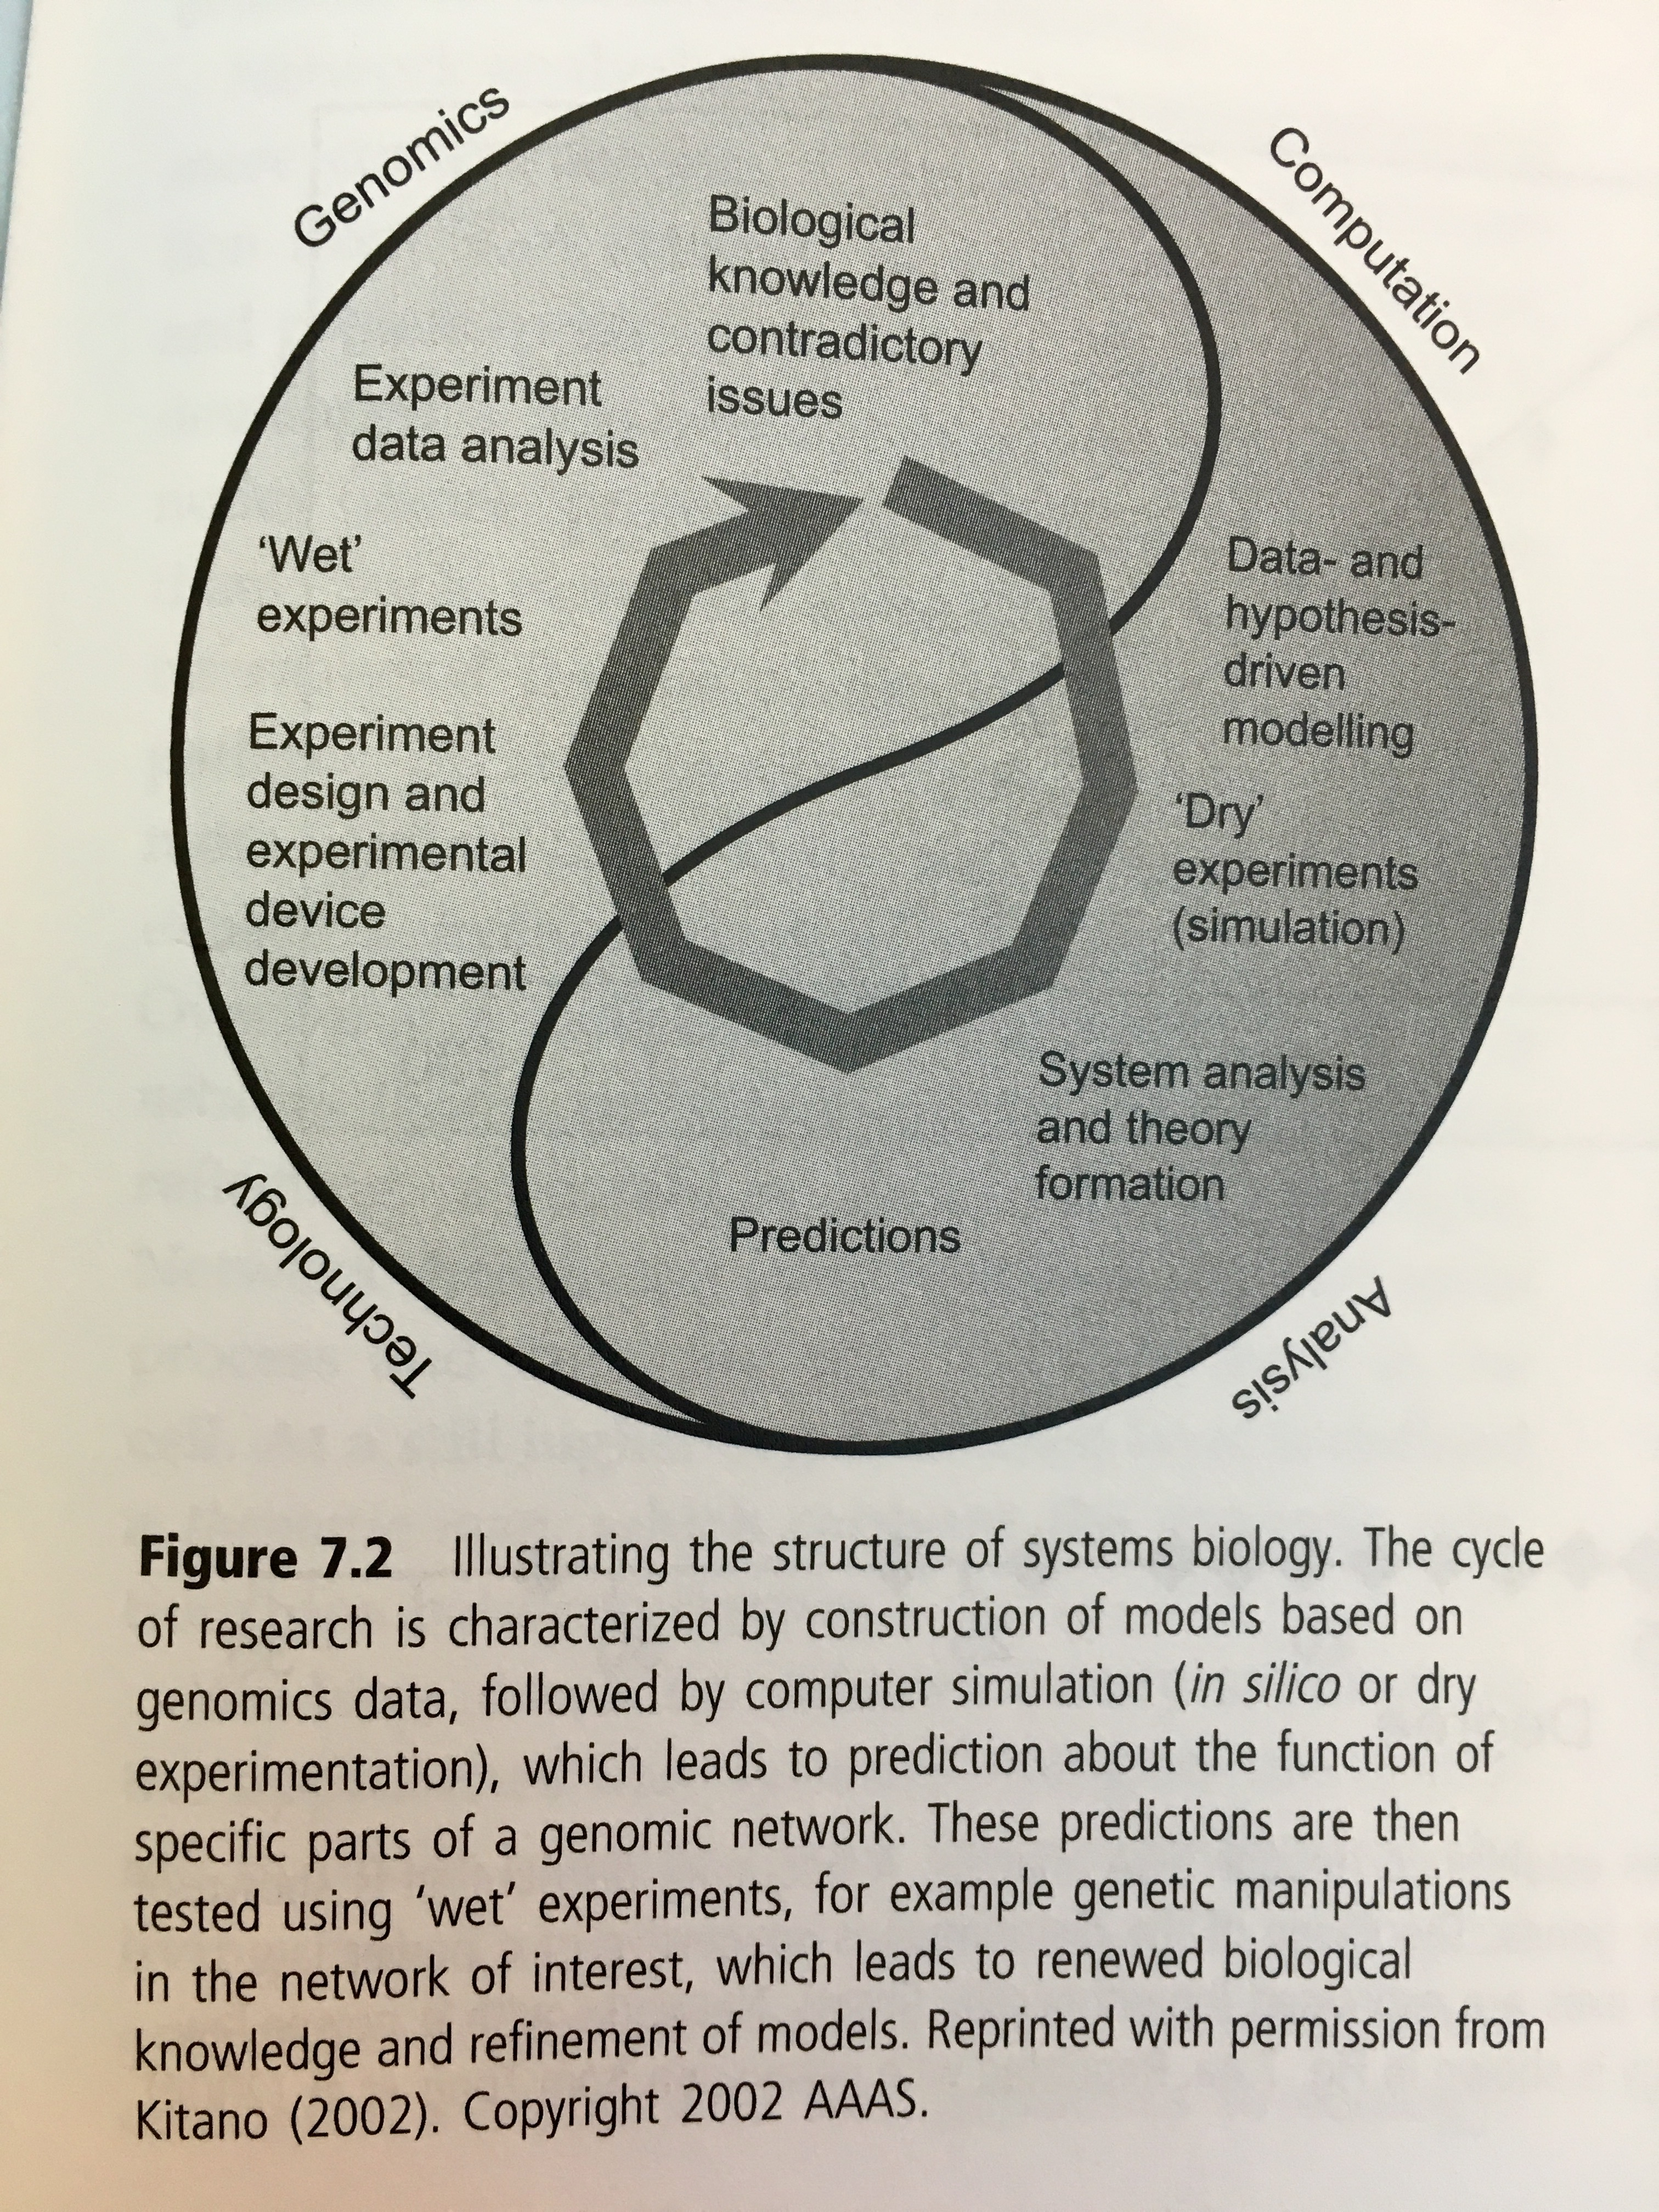
\includegraphics[scale=0.075]{img/ecogenom_fig7_2.jpeg}

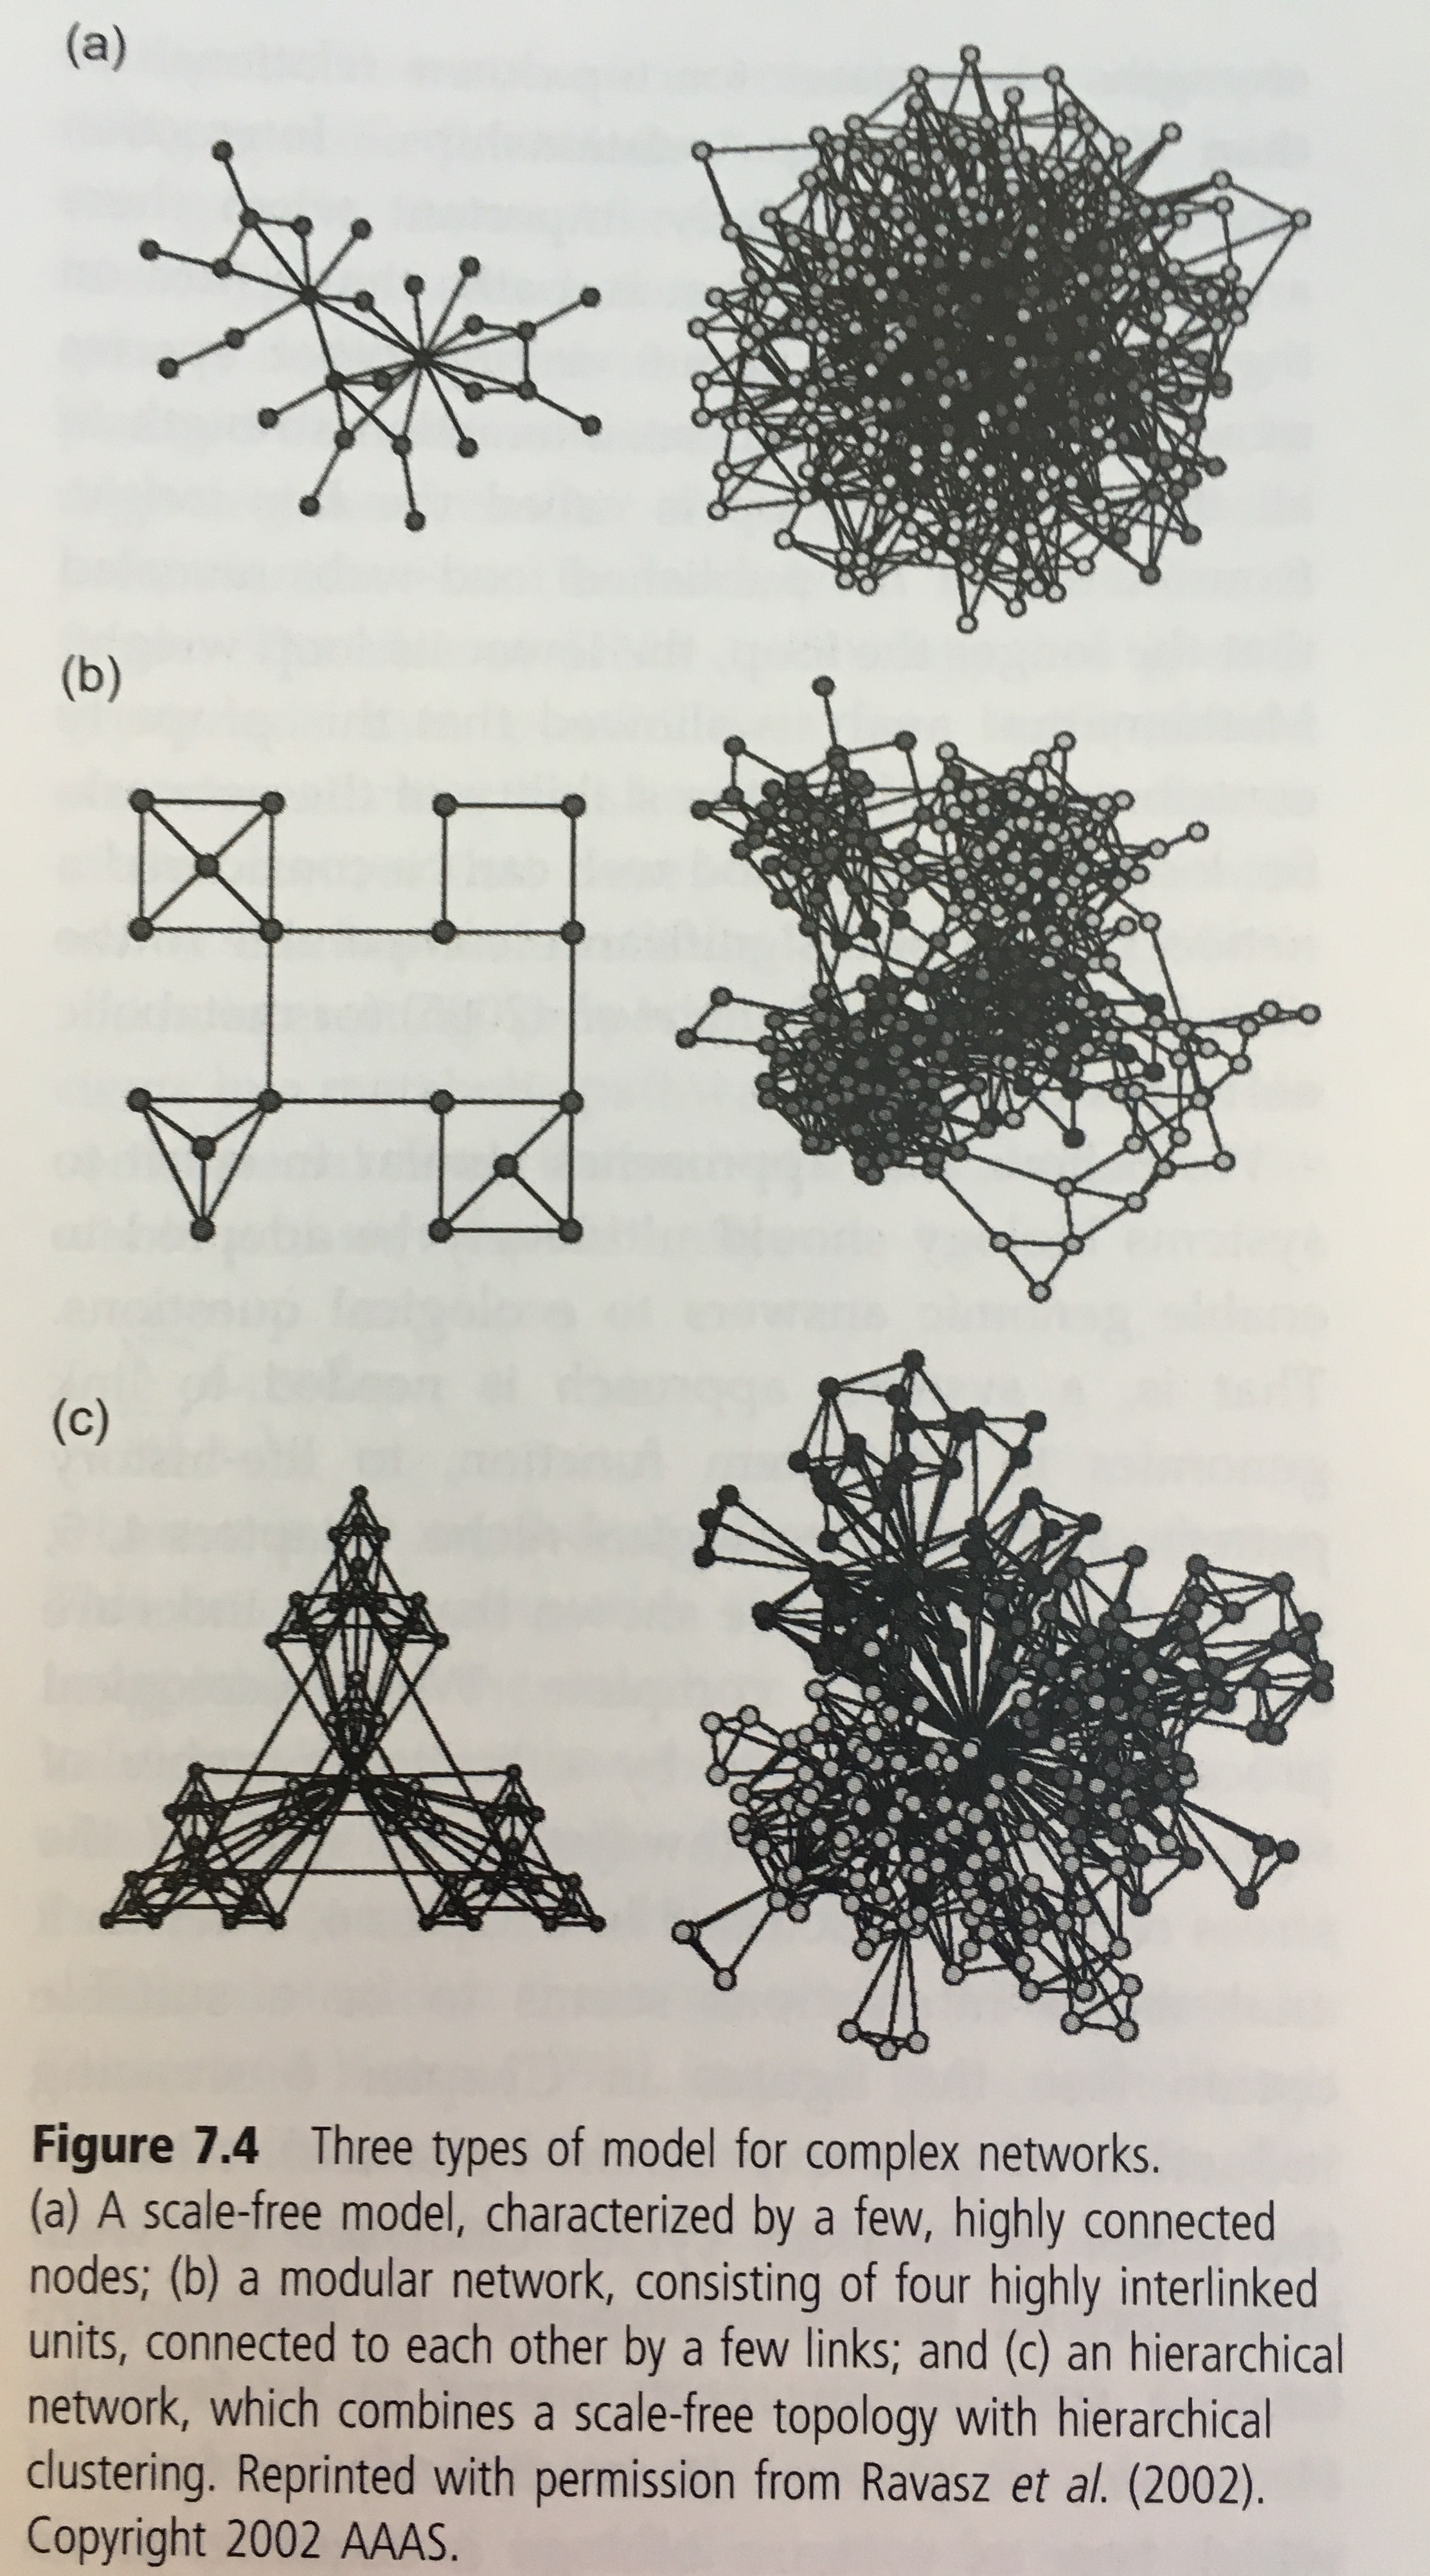
\includegraphics[scale=0.075]{img/ecogenom_fig7_4.jpeg}

\textit{Control Theory}: this is of the same lineage as control theory in ENA

% Bibliography
\bibliography{apGenomes}

\end{document}
